\documentclass[aspectratio=169]{beamer}
\usetheme{metropolis}
\usepackage{kotex}
\usepackage{fontspec}
\usepackage{setspace}
\usepackage{ragged2e}
\usepackage{minted}

\setmonofont[Scale=MatchLowercase]{NanumGothicCoding}
\definecolor{GrayCodeBlock}{RGB}{241,241,241}
\usemintedstyle{manni}
\setminted{fontsize=\small, baselinestretch=1, bgcolor=GrayCodeBlock}


\setmainhangulfont[Mapping=tex-text]{NanumMyeongjo}
\setsanshangulfont[Mapping=tex-text]{NanumGothic}

\usefonttheme{professionalfonts}
\usefonttheme[onlymath]{serif}

\title{Galaxy Watch를 이용한 심박수 측정}
\date{}
\author{
    20205178 박현
}
\metroset{block=fill}

\institute{한림대학교 정보과학대학}

\definecolor{smartleadcolor}{RGB}{29, 61, 111}
\definecolor{smartleadsubcolor}{RGB}{29, 64, 117}
\definecolor{smartleadgray}{RGB}{241, 243, 242}

\definecolor{smartleadbeige}{RGB}{245, 239, 215}
\definecolor{smartleadgreen}{RGB}{228, 240, 235}

\setbeamercolor{frametitle}{bg=smartleadcolor}
\definecolor{themecolor}{RGB}{35, 55, 59}

\setbeamercolor{block title}{bg=smartleadbeige, fg=black}
\setbeamercolor{block body}{bg=smartleadgray}

\setbeamercolor{block title alerted}{bg=smartleadgreen, fg=black}
\setbeamercolor{block body alerted}{bg=smartleadgray}

\begin{document}
    \maketitle
    \begin{frame}{어플리케이션 개요}
        \begin{columns}
            \begin{column}{0.45\linewidth}
                \begin{itemize}
                    \item 심박수 및 가속도/각가속도 측정
                    \item 측정된 결과의 내부 저장 및 FTP 서버로 전송
                \end{itemize}
            \end{column}
            \begin{column}{0.45\linewidth}
                \begin{figure}
                    \centering
                    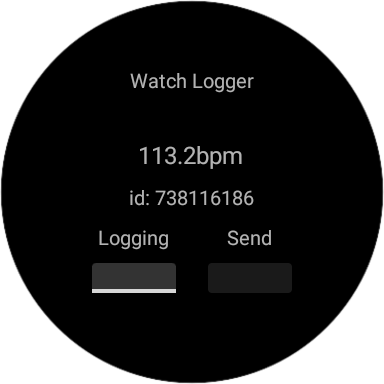
\includegraphics[width=4cm]{Screenshot_20230304_154020.png}
                    \caption{어플리케이션 실행 화면}
                \end{figure}
            \end{column}
        \end{columns}
    \end{frame}
    \begin{frame}{데이터 형식}
        \begin{figure}
            \centering
            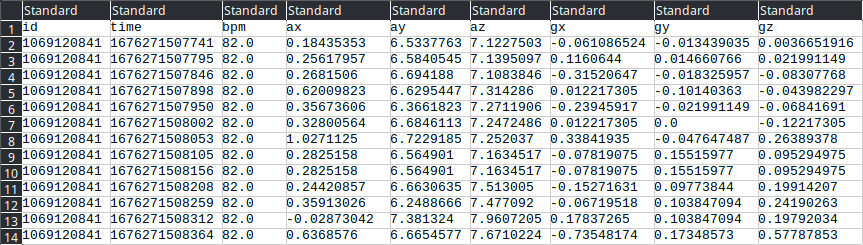
\includegraphics[width=14cm]{Screenshot_20230304_153539.png}
            \caption{Galaxy Watch4로 테스트해본 결과물}
        \end{figure}
    \end{frame}

    \begin{frame}[fragile]
        \frametitle{FTP와의 통신에 문제가 발생 시 예비로 쓸 수 있는 스크립트}
        \begin{minted}{bash}
#!/bin/bash

echo "Watch Logger - File Extractor"
echo "================================================"
adb devices
read -p "Device: " device
echo "================================================"
echo "List of available heart rate log files"
adb -s "$device" exec-out run-as kr.ac.hallym.watchlogger ls files
echo ""
read -p "File: " filename
adb -s "$device" exec-out run-as kr.ac.hallym.watchlogger cat files/"$filename" > "$filename"
echo "================================================"
echo "Successfully extracted."
echo "================================================"
        \end{minted}
    \end{frame}
\end{document}